\documentclass{article}
\usepackage[utf8]{inputenc}
\usepackage[margin=0.5in]{geometry}
\usepackage{tikz}
\usepackage{xcolor}
\usepgflibrary{arrows}
\usetikzlibrary{svg.path}
\usepackage{fancyhdr}
\usepackage{hyperref}
\usepackage{graphicx}
\graphicspath{ {images/} }
\title{CSP203: Project's Test Document}
\author{Naman Goyal (2015CSB1021) \\
Sarthak Gupta (2015CSB1029) \\
Vishal Singh (2015CSB1040) \\
Nittin Singh (2015CSB1067)
}
\begin{document}

\begin{titlepage}
\begin{center}
\vspace{1cm}
\Large{CSP203 - Software Systems Lab}
\vfill

\line(1,0){400}\\[1mm]
\huge{\textbf{Project's Test Document\\IIT Ropar App}}\\
\large{(Version: 1.0)}\\
\line(1,0){400}\\
\vfill
\Large{Naman Goyal (2015CSB1021) \\
Sarthak Gupta (2015CSB1029) \\
Vishal Singh (2015CSB1040) \\
Nittin Singh (2015CSB1067)
}\\

\vfill
\large{\today}\\
\end{center}
\end{titlepage}

\tableofcontents
\clearpage
\usetikzlibrary{positioning,shapes,shadows,arrows}
\definecolor{mycolor}{RGB}{220,150,0}
\definecolor{my2color}{RGB}{150,150,150}
\definecolor{my3color}{RGB}{0,170,220}

\newpage
\section{Introduction}
To ease students' stay at IIT Ropar, and provide one click access to all relevant event updates at the institute.
\section{Unit Test}
The overall design is broken into two main features. The description of these are given in the following subsections. We shall write 3 unit test cases for each listed item.
\subsection{Android App}
 The App has been broken into 4 modules

\subsubsection{Profile Management}
This module has 3 activities- Login, Register, Update Profile. The test includes following

\begin{figure}[h]
    \centering
    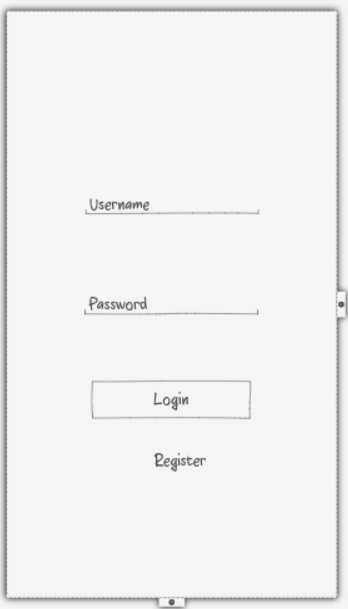
\includegraphics[scale=0.3]{Login.png}
    \caption{Login Page}
\end{figure}

\begin{itemize}
\item[$\bullet$] Create a new user based on type - student, faculty, staff - with an iitrpr email
\item[$\bullet$] Login that User
\item[$\bullet$] Update Profile for User
\item[$\bullet$] Generate Password Reset Link
\item[$\bullet$] Able to store the login info locally on mobile for one-time sign-in support.

\end{itemize}
\subsubsection{Organizer Mode}
This module has 2 activities- CRUD a particular event and List all Organised Events.
\begin{figure}[h]
    \centering
    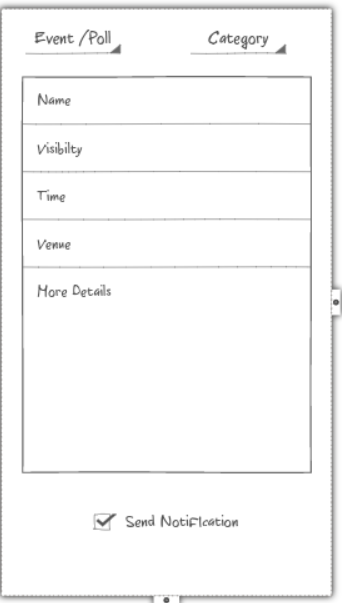
\includegraphics[scale=0.3]{OCRUD.png}
    \caption{Create Event Organizer.png}
\end{figure}


\begin{itemize}
\item[$\bullet$] Able to create a event and poll.
\item[$\bullet$] Able to update, delete that event.
\item[$\bullet$] Able to convert poll from event.
\item[$\bullet$] Able to list all organised events.
\item[$\bullet$] Able to view count of upcoming participant for an organised events.
\end{itemize}
\begin{figure}[h]
    \centering
    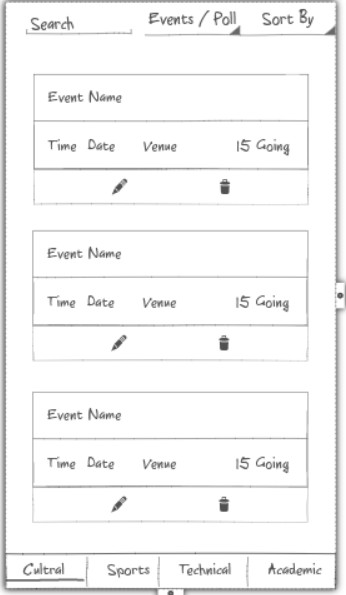
\includegraphics[scale=0.3]{OM.png}
    \caption{Organizer List}
\end{figure}
\subsubsection{User Mode}
This module has 2 activities- 

\begin{figure}[h]
    \centering
    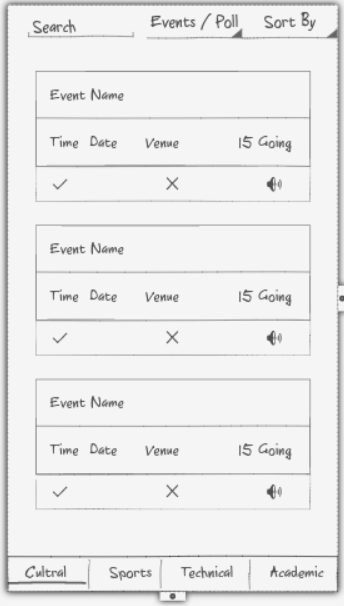
\includegraphics[scale=0.3]{UV.png}
    \caption{List and Sort all Events}
\end{figure}
\begin{enumerate}
\item {List all Events}
\begin{itemize}
\begin{figure}[h]
\centering
    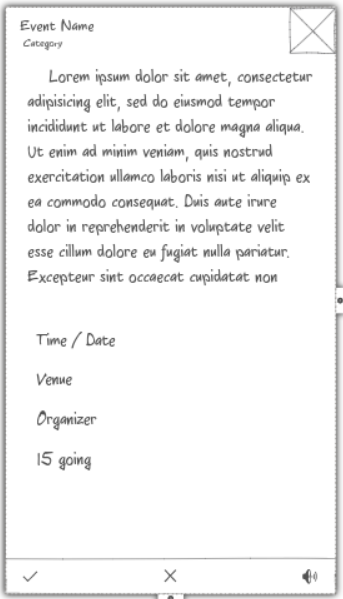
\includegraphics[scale=0.3]{Event.png}
    \caption{Event Details View}
\end{figure}
\begin{figure}[h]
\centering
    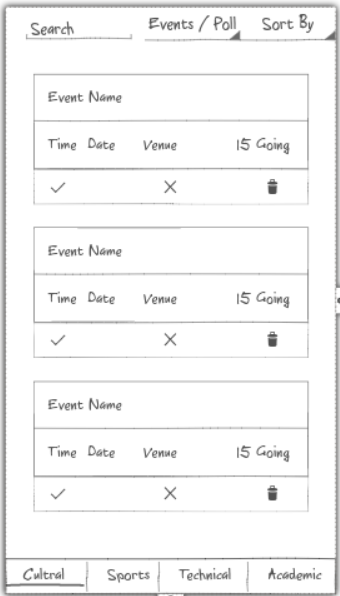
\includegraphics[scale=0.3]{UM.png}
    \caption{Manage Interested Events - User ``Entry"}
\end{figure}
\item[$\bullet$] Able to list all events.
\item[$\bullet$] Able to sort events based on popularity, newly added, date.
\item[$\bullet$] View event based on category - Cultural, Sports, technical, Academic.
\item[$\bullet$] Listed event all only based on type - public for all and rest visible only to that type -  student, faculty, staff
\end{itemize}

\item{CRUD his``entry"}

\begin{itemize}
\item[$\bullet$] Able to create his entry - Going, Not-Going, Notify.
\item[$\bullet$] Able to RUD his entry for an event.
\item[$\bullet$] Able to set notification and calender reminder for interested event i.e. (Going + Interested)
\end{itemize}
\end{enumerate}
\subsubsection{Guest Mode}
Able to list all public events.
\clearpage
\subsection{PHP + mySQL}
The mySQL databale has 3 table consists 
\begin{enumerate}
\item{Users - Store user profile} 
\item{Events - Store all event related details with organizer id}
\item{Entry - Store entry for a user-id for an event-id} 
\end{enumerate}
Now their are php scripts to access and update these data
\subsubsection{Login.php}
Able to authenticate login for a user-id.
\subsubsection{Register.php}
Able to register a new user having unique email iitrpr email.
\subsubsection{ReadProfile.php}
Able to retrieve profile details of user-id.
\subsubsection{Update.php}
Able to update profile details of user-id.
\subsubsection{Password.php}
Able to generate forget password link.
\subsubsection{List-Event.php}
Able to retrieve all organised event info for an event in sql table for a organizer-id, category, type based on user-id.

\subsubsection{Read-Event.php}
Able to retrieve details for an event in sql table.
\subsubsection{Create-Event.php}
Able to create new row for an event in sql table for a organizer-id.
\subsubsection{Update-Event.php}
Able to update info for an event in sql table, organizer-id is correct.
\subsubsection{Delete-Event.php}
Able to delete info for an event in sql table, organizer-id is correct.

\subsubsection{Create-Entry.php}
Able to create new Entry in sql table for user-id and event-id.
\subsubsection{Read-Entry.php}
Able to read an Entry in sql table for user-id and event-id.
\subsubsection{Update-Entry.php}
Able to update an Entry in sql table for user-id and event-id.
\subsubsection{Delete-Entry.php}
Able to delete an Entry in sql table for user-id and event-id.

\section{System Test}
When whole module is integrated a user should be to perform all actions synchronously.  We plan to write 10 cases. The cases test interactions of all the module where php scripts are called by volley in android which in then processed by the app.\\
There will be 3 kinds of tests -
\begin{itemize}
\item{A test where a create a register, forgets password, login using app and update his/her profile.}
\item{After login able to view events and CRUD his entry for his event. For e.g. In particular test multiple events will be created and user will test categorization and sorting.}
\item{Based on his entry will the phone reminders and notification be set.}
\item{The user can act as organizer and CRUD event. For e.g. The organizer is able to push event notification and able to prune the target audience.}
\end{itemize}



\end{document}
